\documentclass[10pt,a4paper]{scrartcl}
\usepackage[utf8]{inputenc}
\usepackage{ngerman}
\usepackage{graphicx}
\usepackage[final]{listings}
\lstset{tabsize=2,basicstyle=\ttfamily\small}
\usepackage[draft]{fixme}
\usepackage{color}
\definecolor{LinkColor}{rgb}{0.0,0.0,0.0} 
\usepackage[
        bookmarks=true,
        bookmarksopen=true,
        bookmarksopenlevel={1},
        bookmarksnumbered=true,
        plainpages=false,
        pdfpagelabels=true,
        hypertexnames=false,
        pdftitle={},
        pdfauthor={Sven Wenzel},
        pdfcreator={LaTeX with hyperref and KOMA-Script},
        pdfsubject={},
        pdfkeywords={},
        final]{hyperref}
\hypersetup{colorlinks=true,
        anchorcolor=LinkColor,
        linkcolor=LinkColor,
        citecolor=LinkColor,
        filecolor=LinkColor,
        menucolor=LinkColor,
        pagecolor=LinkColor,
        urlcolor=LinkColor}

\newcommand{\hinweis}[1]{

\textbf{Hinweis:} #1

}

\title{Introduction to SiDiff 2.0\\Compare Functions}
\author{Timo Kehrer, Pit Pietsch}
\begin{document}
\maketitle
\tableofcontents
\newpage
\section*{Dokumenthistorie}
Dieses Dokument wird fortlaufend gepflegt. Die nachfolgende Tabelle gibt 
eine Übersicht über die Änderungen in einzelnen Versionen.\\


\noindent
\begin{tabular}{|c|p{11cm}|}\hline
Datum & Änderungen \\\hline\hline
07.09.09 & erste Version (Grobstruktur) \\\hline
11.09.09 & erste vollständige Version \\\hline
\end{tabular} 


\newpage


\section{About this Document}
Vergleichsfunktionen sind ein elementarer Bestandteil von SiDiff. In diesem Dokument wird zunächst
der Einsatzkontext sowie die prinzipielle Funktionsweise von Vergleichsfunktionen beschrieben.
Nach einer kurzen Betrachtung einfacher Vergleichsfunktionen wird ein mächtiger Mechanismus
zur Komposition und Konfiguration komplexer Vergleichsfunktionen mittels Komparatoren beschrieben. 
Anschließend wird das Konzept der bedingten Vergleichsfunktionen betrachtet.
Abschließend folgt eine Übersicht über die in SiDiff vorhandenen Vergleichsfunktionen und Komparatoren.



\section{Introduction}
\label{introduction}
The similarity computation is one of the key features of SiDiff. SiDiff supports the definition of
arbitrary similarity heuristics to determine whether two model elements correspond or not. 
The heuristics are given by configuration files that define comparison rules for each type of
element.

\subsection{Comparison Rules}
\label{comparison-rules}
A comparison rule defines the element properties which are relevant for the similarity of two
elements of the same type (i.e. elements that are instances of the same class in the metamodel). 
The properties are either local attributes (e.g.~names) or other elements in the neighborhood.


Each compare function returns a value between 0.0 and 1.0; a value of 0.0 stands for no similarity
between the properties, a value of 1.0 expresses equality. The comparison rules assign each property
with a weight indicating the relevance of the property for the similarity of two elements.
Further, each comparison rule specifies a threshold, i.e. a minimum similarity for two elements of
this type to be eligible as corresponding elements.

More formally, the similarity between two elements is defined as the weighted arithmetic mean of the
similarities of the similarity-relevant properties.
\[ sim_{e_1,e_2} = \sum_{p \in P} w_p \cdot \mathrm{compare_p(e_1, e_2)}, \]
where $e_1$ and $e_2$ are the elements to be compared, $P$ is the set of
similarity-relevant properties, $w_p$ gives the weight of property $p$ and
$compare_p$ is the compare function (see Section \ref{compare-functions}) for property $p$. 

\subsection{Compare Functions}
\label{compare-functions}
According to the formula introduced in Section \ref{comparison-rules}, the comparison rules assign
a compare function to each property considered for the similarity. SiDiff provides several compare
functions. A very simple example is a compare function that simply checks whether the model elements
that should be compared are equal (cf. Section \ref{trivial-functions}).

Generally, a compare function takes two model elements, one from model A and one from model B, as
input and returns a value between 0.0 and 1.0. A value of 1.0 means that both model elements are 
identical with respect to the property that is considered by a specific compare function. A value
of 0.0 means that both model elements have no similarity with respect to a specific property.


\subsection{Configuration File}
Comparison rules and compare functions are defined within a configuration file. The follwoing listing
shows a very simple configuration rule containing exactly one trivial compare function (cf. Section 
\ref{trivial-functions}):

\begin{lstlisting}
<Class name="PrimitiveType" threshold="1.0">
	<CompareFunction class="Equality" weight="1.0"/>
</Class>
\end{lstlisting}

The example is taken from a configuration file for UML models. The comparison rule states, that 
model elements of type PrimitiveType should be compared with respect to a trivial property: equality.
The threshold for this comparison rule is 1.0; two elements of type PrimitiveType can only correspond
if they are equal.

The actual comparison with respect to equality is done by a compare function called Equality. 
The weight of the compare function is of course 1.0 because it is the only compare function used by
this comparison rule. In case of complex compare functions, these can be further configured by means
of an additional parameter string. For further information on the available parameters and the
syntactical structure of the parameter, please refer to the JavaDoc of the respective compare function.


\subsection{Compare Function Interface}
Die Schnittstelle von Vergleichsfunktionen ist seh einfach aufgebaut. Sie besteht aus einem Anteil zur
Konfiguration und der eigentlichen Methode zur Berechnung der Ähnlichkeit zwischen zwei Modellelementen.
Da zur Repräsentation von Modellen in Sidiff das Eclipse Modeling Framework (EMF, s. WhitePaper ``Introduction to
Modelmanagement'') eingesetzt wird, werden Modellelemente als Instanz der EMF-Klasse \textit{EObject} repräsentiert.
Die Initialisierung wird während der Instanziierung von Vergleichsfunktionen durchgeführt. 
Jede Vergleichsfunktion ist von der abstrakten Klasse CompareFunction abzuleiten.


% Die Ähnlichkeit zweier Modellelemente wird in SiDiff anhand der Eigenschaften dieser Modellelemente
% bestimmt. Dabei werden ausschließlich Elemente gleichen Typs (also Instanzen der gleichen Klasse 
% des Metamodells) miteinander verglichen. Der Wertebereich der errechneten Ähnlichkeit liegt zwischen
% 1.0 (identisch) und 0.0 (keine Ähnlichkeit).
% 
% 
% Zu der Ähnlichkeit zweier Modellelemente können dabei verschiedenste Eigenschaften beitragen.
% Die errechnete Gesamtähnlichkeit zweier Modellelemente ergibt sich dabei als die gewichtete Summe 
% einer Menge von elementaren Ähnlichkeitswerten dieser Modellelemente. Vergleichsfunktionen dienen
% der Berechnung von elementaren Ähnlichkeitenswerten.
% 
% 
% Die einem Vergleich zu Grunde liegende Heuristik kann über eine Konfigurationsdatei spezifiziert
% werden. Für jeden Typ (d.h. jede Klasse des Metamodells) werden dabei die zu vergleichenden elementaren
% Eigenschaften (d.h. die zu verwendenden und deren Gewichtung festgelegt


\section{Trivial Compare Functions}
\label{trivial-functions}
In Abschnitt \ref{complex-functions} wird ein sehr mächtiger Mechanismus zur Realisierung von Vergleichsfunktionen
eingeführt. Dabei werden konfigurierbare Komparatoren benutzt, um komplexe Vergleichsfunktionen
wie bspw. den Vergleich einer bestimmten Eigenschaft aller Kindelemente zweier zu vergleichender
Modellelemente zu realisieren. Als triviale Vergleichsfunktionen hingegen bezeichnen wir solche 
Vergleichsfunktionen, die nicht nach diesem Mechanismus aufgebaut sind.

Dies ist dann der Fall, wenn es sich um sehr spezielle, nicht weiter konfigurierbare
Vergleichsfunktionen für einen ganz bestimmten Einsatzkontext handelt, oder die zu vergleichende 
Eigenschaft sehr einfach ist. In Abschnitt \ref{introduction} wurde bereits die Eigenschaft der
Gleichheit als ein Vertrteter trivialer Vergleichsfunktionen eingeführt. Weitere Beispiele sind
\texttt{MaximumSimilarity} und \texttt{NoSimilarity} welche stets die Werte 1.0 bzw. 0.0 als 
Ähnlichkeit für zwei Modellelemente des gleichen Typs zurückliefern.



\section{Komplexe Vergleichsfunktionen}
\label{complex-functions}

In den Absschnittn \ref{modularisation} und \ref{comparators} wird der prinzipielle Aufbau und die
Konfiguration komplexer Vergleichsfunktionen beschrieben. 
Zur anschaulichen Erläuterung dient das in Abschnitt \ref{ref-example} eingeführte Beispiel.


\subsection{Einführendes Beispiel}
\label{ref-example}
Als Beispiel soll eine Vergleichsfunktionen dienen, welche zwei Modellelemente anhand iher Kindelemente
vergleicht. Wir gehen davon aus, dass die Kindelemente geordnet sind. Der Vergleich der beiden
Listen soll mittels LCS durchgeführt werden. Basis des Vergleichs einzelner Kindelemente
im Rahmen des LCS soll eine lokale Eigenschaft der Kindelemente, hier als Attribut bezeichnet,
darstellen. Der Datentyp des Attributwerts entscheidet schließlch darüber, wie die Attributwerte
miteinander verglichen werden sollen. In unserem Fall soll ein einfacher String-Vergleich ohne
Beachtung von Groß- und Kleinschreibung durchgeführt werden.

\subsection{Modularisierung durch Trennung der Aspekte WAS und WIE}
\label{modularisation}

Wir beschreiben im Folgenden sowohl die konzeptuelle Unterscheidung der beiden Aspekte
WAS und WIE, als auch die Realisierung der Unterscheidung im Rahmen von SiDiff.

\subsubsection{Konzeptuelle Unterscheidung}
Zunächst stellt sich bei der Realisierung komplexer Vergleichsfunktionen
die Frage, WAS miteinander verglichen werden soll. So z.B. 
\begin{itemize}
	\item lokale Eigenschaften,
	\item die Kindelemente,
	\item die Elternelemente,
	\item über einen Pfadausdruck erreichbare Modellelemente,
	\item etc.
\end{itemize}
der zu vergleichenden Modellelemente. In dem in Abschnitt \ref{ref-example} eingeführten Beispiel 
besteht der WAS-Aspekt also aus den beiden geordneten Listen der Kindelemente.

Zusätzlich zur Frage, WAS im Kontext einer Vergleichsfunktion für den Vergleich zweier
Modellelemente herangezogen werden soll muss spezifiziert werden, WIE die ausgewählten lokalen
Eigenschaften bzw. Modellelemente zu vergleichen sind. In unserem Referenzbeispiel muss spezifiziert
werden, WIE die Kindelelemente miteinander verglichen werden.

\subsubsection{Realisierung in SiDiff}
Zur Selektion der zu vergleichenden Modellelemente oder Attributwerte existiert in SiDiff bereits eine
Menge von \textit{Vergleichsfunktionen} (s. Abschnitt \ref{existing-functions}). Es ist zu beachten, 
dass der Begriff \textit{Vergleichsfunktion} an dieser Stelle überladen wird. Bisher wurde in diesem
Dokument unter einer Vergleichsfunktion eine Funktion zum Vergleich zweier Modellelemente auf Basis
bestimmter Eigenschaften verstanden, welche die Aspekte WAS und WIE gleichermaßen umfasst. Hier führen
wir die Vergleichsfunktion als funktionalen Bestandteil einer gesamten Vergleichsfunktion ein, welcher
lediglich die Selektion der zu vergleichenden Elemente bzw. Attributwerte, also den WAS-Aspekt, umfaßt.
Die jeweilige Bedeutung des Begriffs Vergleichsfunktion sollte sich anhand des Kontexts erschließen lassen.

WIE die selektierten Modellelemente bzw. Attributwerte miteinander zu vergleichen sind
wird an weitere funktionale Einheiten delegiert; die Komparatoren. Deren Aufbau und Konfiguration
werden im Folgenden näher betrachtet.


\subsection{Komparatoren}
\label{comparators}
In diesem Abschnitt werden die prinzipielle Funktionsweise sowie die Konfiguration von Komparatoren 
beschrieben.

\subsubsection{Prinzipielle Funktionsweise}
Die Dekomposition in kleine, funktionale Einheiten, sowie die hierarchische Schachtelung
von Komparatoren ist das Kernprinzip der SiDiff-Komparatoren.
Ähnlich wie Vergleichsfunktionen den eigentlichen Vergleich zweier selektierter Eigenschaften an
Komparatoren delegieren, können auch Komparatoren Teile des Vergleichs wieder an weitere Komparatoren
delegieren.

Jeder Komparator erfüllt dabei eine klar definierte, abgeschlossene Aufgabe. Komplexe Vergleiche
lassen sich durch die Komposition von Komparatoren zu einer Art Pipeline realisieren. Zur Realisierung
des eigentlichen Vergleichs der Kindelemente in unserem Referenzbeispiel lassen sich bspw. folgende
Komparatoren einsetzen: Zunächst führt ein Komparator zum abstrakten Vergleich von Listen nach dem
LCS-Prinzp den Verleich der Beiden Listen durch. Um die Ähnlichkeit der in den Listen enthaltenen 
Modellelemente zu bestimmen, wird ein weiterer Komparator benutzt, hier ein Komparator zum Vergleich
von lokalen Attributen. Dieser wiederum kann den eigentlichen Wertevergleich der lokalen Attribute an einen
weiteren Komparator abhängig vom Typ (numerisch, String, etc.) der zu vergleichenden Werte delegieren.
Hier wird ein Komparator zum case-insensitiven Vergleich von String-Werten eingesetzt.

Ähnlich wie Vergleichsfunktionen den eigentlichen Vergleich zweier selektierter Eigenschaften an
Komparatoren delegieren, können auch Komparatoren Teile des Vergleichs wieder an weitere Komparatoren
delegieren. So z.B. den Vergleich zwei Listen von Modellelementen. Eine typische Konfiguration
spezifiziert einen Komparator, der ein Verfahren zum abstrakten Vergleich von Listen realisert,
so z.B. nach dem LCS-Prinzip. Um die Ähnlichkeit der in den Listen enthaltenen Modellelemente
zu bestimmen, wird ein weiterer Komparator benutzt, z.B. ein Komparator zum Vergleich von lokalen
Eigenschaften. Dieser wiederum kann den eigentlichen Wertevergleich der lokalen Attribute an einen
weiteren Komparator abhängig vom Typ (numerisch, String, etc.) der zu vergleichenden Werte delegieren.


\subsubsection{Konfiguration und Anpassung}
\label{comparator-configuration}
Die Mächtigkeit des Komparator-Konzepts besteht in der Konfiguration sowie der hierarchischen
Schachtelung von Komparatoren im Rahmen der Konfigurationsdatei. Das folgende Listing bezieht sich
auf das im Verlauf dieses Kapitels behandelte Referenzbeisbiel.

\begin{lstlisting}
<CompareFunction class="ChildrenCF" weight="0.2" 
	parameter="LCLongestCommonSubsequence[
		ECAttributeStatic[VCString[ci];SomeType;someAttributeName];0.6
	]"/>
\end{lstlisting}

Komparatoren werden, wie auch Vergleichsfunktionen, über einen Parameter-String konfiguriert. Die
einzigen syntaktischen Elemente eiens Parameter-String sind das Semikolon (``;'') sowie die eckigen
Klammern (``['' und ``]''). Eckige Klammern umfassen den Parameter-String eines Komparators, das 
Semikolon trennt einzelne Segmente eines solchen Parameter-Strings voneinander ab. Im dargestellten
Beispiel wird als erster Komparator in der Pipeline der LCLongestCommonSubsequence benutzt.
Dieser erwartet offenbar vier Parameter: Einen weiteren Komparator (hier: ECAttributeStatic) und 
einen numerischen Wert (hier: 0.6). Bei dem numerischen Wert handelt es sich um einen Threshold, 
dessen genaue Bedeutung der Code-Dokumentation der Klasse LCLongestCommonSubsequence zu entnehmen ist.
Der Komparator ECAttributeStatic erwartet drei Parameter: den konkreten Komparator zum Vergleich
der Attributwerte (hier: Ein String-Komparator (VCString) unter Nichtbeachtung von Groß- und 
Kleinschreibung\footnote{der Parameter ci steht für case-insensitive, s. auch JavaDoc}), eine
Typinformation der zu vergleichenden Elemente (hier: SomeType) sowie den Namen des zu vergleichenden
Attributs (hier:someAttributeName).


\subsubsection{Die Komparator-Schnittstelle}
Die Schnittstelle von Komparatoren ist ähnlich aufgebaut wie die der Vergleichsfuntionen.
Sie besteht aus einem Anteil zur Initialisierung des Komparators sowie einer Methode zur
Durchführung des eigentlichen Vergleichs. Im Gegensatz zu Vergleichsfunktionen werden hier jedoch
nicht zwangsläufig zwei Modellelemente (also Instanzen der EMF-Klasse EObject), sondern beliebige
Java-Objekte übergeben. So z.B. Attributwerte, Listen von Modellelementen, Modellelemente etc.


\section{Bedingte Vergleichsfunktionen}
\textbf{TODO:} Future Work


\section{Existierende Vergleichsfunktionen und Komparatoren}

\subsection{Allgemeines}
\label{existierende-allgemeines}
Eine Unterscheidung von Vergleichsfunktionen konzeptueller Natur ist die bereits beschriebene
Unterscheidung von trivialen (s. Abschnitt \ref{trivial-functions} und komplexen 
Vergleichsfunktionen (s. Abschnitt \ref{complex-functions}).

Weiterhin lassen sich die verschiedenen Vergleichsfunktionen anhand eines technischen Merkmals
unterscheiden: der Abhängigkeiten zu anderen SiDiff-Komponenten (OSGI-Bundles). 
Um die Abhängigkeit zu anderen Bundles bei der Konfiguration von SiDiff-Applikationen
möglichst auf ein Minimum zu reduzieren haben wir uns dazu entschlossen, die Vergleichsfunktionen
anhand ihrer Abhängigkeit zu anderen SiDiff-Komponenten auf verschiedene Bundles zu verteilen.
Momentan existierende folgende Bundles:



\begin{itemize}
\item \texttt{org.sidiff.core.compare.comparefunctions}:\\
	Vergleichsfunktionen ohne jegliche Abhängigkeiten zu anderen Bundles. Insbesondere fallen
	unter diese Kategorie Vergleichsfunktionen ohne Modellzugriff, so z.B. die in Abschnitt
	\ref{trivial-functions} bereits angesprochene Vergleichsfunktion \texttt{MaximumSimilarity}.
	Alle folgenden Vergleichsfunktionen greifen auf die Modelle zu.
\item \texttt{org.sidiff.core.compare.comparefunctions.emf}:\\
	Ausschließlich EMF-spezifische Vergleichsfunktionen
\item \texttt{org.sidiff.core.compare.comparefunctions.emf.annotations}:\\
	Vergleichsfunktionen welche Annotationswerte auslesen
\item \texttt{org.sidiff.core.compare.comparefunctions.emf.correspondence}:\\
	Vergleichsfunktionen auf Basis von Korrespondenzen
\item \texttt{org.sidiff.core.compare.comparefunctions.emf.similarity}:\\
	Vergleichsfunktionen auf Basis von Ähnlichkeiten
\item \texttt{org.sidiff.core.compare.comparefunctions.emf.correspondenceandsimilarity}:\\
	Vergleichsfunktionen welche die Korrespondenz- und die Ähnlichkeitstabelle benutzen
\end{itemize}


\subsection{Vergleichsfunktionen}
\label{existing-functions}

\paragraph{Triviale Vergleichsfunktionen}
Die in SiDiff vorhandenen, trivialen Vergleichsfunktionen wurden bereits in Abschnitt 
\ref{trivial-functions} vollständig aufgeführt und sollen hier nicht weiter betrachtet werden.


\paragraph{Vergleichsfunktionen zur Verwendung in Verbindung mit Komparatoren}
Abb. \ref{available-compare-functions} liefert einen Überblick über die in SiDiff verfügbaren 
Vergleichsfunktionen, welche in Verbindung mit Komparatoren eingesetzt werden können. 
Diese Vergleichsfunktionen erfüllen den
in Abschnitt \ref{modularisation} beschriebenen WAS-Aspekt bei der Realisierung komplexer Vergleichsfunktionen.
Ihre primäre Aufgabe besteht also darin, lokale Eigenschaften oder Elementmengen bzw. -listen
zu berechnen und die den weiteren Vergleich an Komparatoren zu delegieren.
Die Semantik der jeweiligen Vergleichsfunktionen ist der JavaDoc der entsprechenden Bundles 
(s. Abschnitt \ref{existierende-allgemeines}) zu entnehmen.

\begin{figure}[htb]
	\begin{center}
 		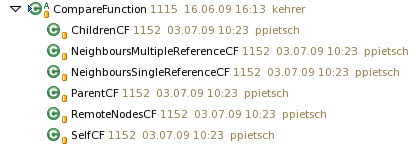
\includegraphics[scale=1.0]{pics/available-compare-functions.png}
	\end{center}
	\caption{Verfügbare Vergleichsfunktionen zur Verwendung in Verbindung mit Komparatoren}
	\label{available-compare-functions}
\end{figure} 


\subsection{Komparatoren}
SiDiff stellt bereits einige Komparatoren für verschiedenste Einsatzzwecke zur Verfügung. Eine
detailiierte Übersicht über alle Komparatoren und deren Funktionsweise ist dem
Dokument CompareFunctionsJavadoc.pdf zu entnehmen. Abb.
\ref{available-comparators} zeigt eine kurze Übersicht. Es ist dabei zu
beachten, dass es sich lediglich bei den Blättern der in Abb.
\ref{available-comparators} dargestellten Vererbungshierarchie um konkrete
Komparatoren handelt. Alle anderen Komparatoren sind abstrakt und dienen
lediglich einer Klassifizierung der Funktionsweise der Komparatoren.

\begin{figure}[htb]
	\begin{center}
 		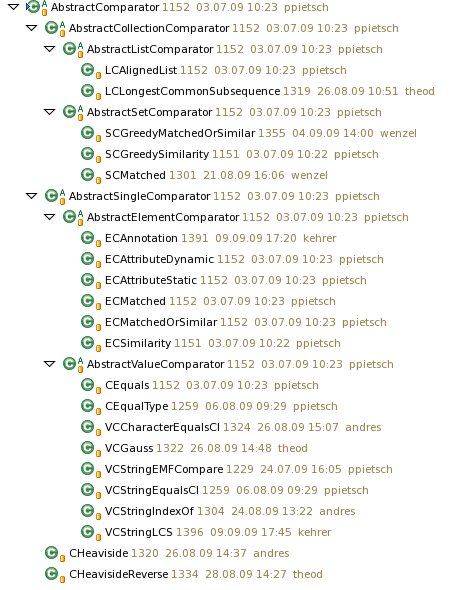
\includegraphics[scale=1.0]{pics/available-comparators.png}
	\end{center}
	\caption{Verfügbare Komparatoren in SiDiff}
	\label{available-comparators}
\end{figure} 

\textbf{TODO:} Hier sollten wohl eher die einzelnen Kategorien und deren Intention näher beschrieben
werden, als einfach nur die vorhandenen Komparatoren abzubilden!?

\end{document}
